\section{Sharing work through workshares}

%The parallelism in an OpenMP application program is expressed through
%parallel regions, worksharing constructs, and combined parallel
%constructs. A combined parallel construct can be considered as a
%parallel region with only one worksharing construct inside it,
%although its implementation may be more efficient from a performance
%point of view. In any case, a parallel region is the basic concept
%in OpenMP programming.

When a \texttt{parallel} region starts, multiple threads will execute the code
inside the region concurrently,

\begin{figure}[!h]
  \begin{center}
    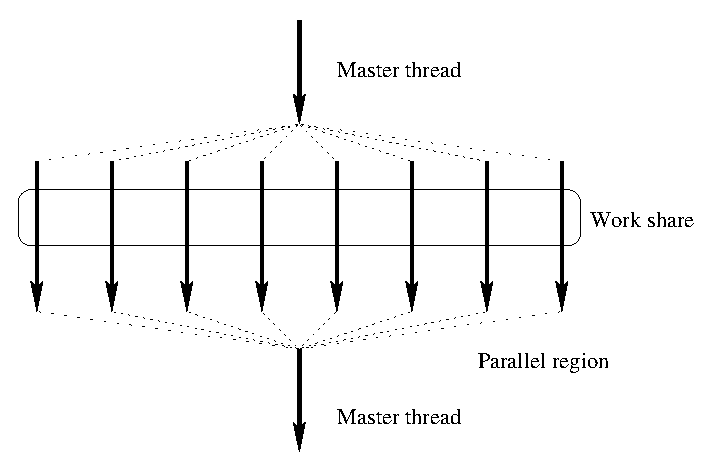
\includegraphics[angle=0, width=0.65\textwidth]{parregion.eps}
    \caption{\footnotesize Parallel region}
    \label{fig:parregion}
  \end{center}
\end{figure}

In Figure \ref{fig:parregion}, a master thread starts up the \texttt{parallel}
region executed by 8 threads. Through parallel regions, multiple threads
accomplish \emph{worksharing} in an OpenMP program.

The simplest format of worksharing is replicated execution of the same code
segment on different threads. It is more useful to divide work among multiple
threads --- either by having different threads operate on different portions of
a shared data structure, or by having different threads perform entirely
different tasks. Each cooperation of this kind is considered as a
\emph{workshare}\footnote{The concept of workshare here is different from the
parallel construct, \texttt{WORKSHARE} in Fortran OpenMP specification 2.0,
which can be treated semantically as the combination of \texttt{for} and
\texttt{single} constructs.} in this paper. In the Figure \ref{fig:parregion}, we use a
round-cornered rectangular block to represent one workshare.

The most common forms of workshares in OpenMP specification are \texttt{omp for} 
and \texttt{omp sections},

%as shown in Figure \ref{fig:workshare} (a) and (b) respectively.
%
%\begin{figure}[!h]
%  \begin{center}
%    \includegraphics[angle=0, width=0.6\textwidth]{workshare.eps}
%    \caption{\footnotesize Common workshare}
%    \label{fig:workshare}
%  \end{center}
%\end{figure}
%
%We use different numbers to mark the sequential order of the blocks in an
%OpenMP \texttt{for} construct, but it does not mean the implementation will
%ensure that the corresponding threads will work on those blocks. In fact, the
%mapping of work to threads is determined by the schedule type of the
%\texttt{for} construct as specified by the OpenMP standard. Similarly, the
%mapping between the sections in a \texttt{sections} construct and the threads
%is also decided by the schedule type. The fundamental difference between a
%\texttt{for} construct and a \texttt{sections} construct is that in a
%\texttt{sections} region the code segments executed by threads could be
%entirely different.

%Besides the common workshares introduced above, 

%The typical examples are
%\texttt{single} constructs and explicit barriers, as in Figure
%\ref{fig:synchronization} (a) and (b).
%
%\begin{figure}[!h]
%  \begin{center}
%    \includegraphics[angle=0, width=0.6\textwidth]{synchronization.eps}
%    \caption{\footnotesize Synchronization workshare}
%    \label{fig:synchronization}
%  \end{center}
%\end{figure}

We can also consider OpenMP \texttt{single} as a special workshare too.  A
\texttt{single} construct is semantically equivalent to a \texttt{sections}
construct with only one \texttt{section} inside.  For a \texttt{single}
construct, the first thread that encounters the code will execute the block.
This is different from a \texttt{master} construct, where the decision must be
made by checking the thread id.

All the workshares introduced here have an important common feature: they have
an implicit barrier at the end of the construct, which may be disabled by using
the optional \texttt{nowait} clause. Besides, An explicit \texttt{barrier}
region is semantically equivalent to an empty workshare without the
\texttt{nowait} clause. 

This observation reveals that the barrier is the most important workshare to in
a runtime supporting system. We will discuss more about a barrier
implementation in the next section.

Different implementations may have a different kind of classification. The real
advantage of considering them all as workshares is for simplifying the
developing process. From an implementation point of view, the common behaviors
will lead to a common code base, thus improving the overall code quality. And
once we have a barrier implementation on Cell, the implementation of the rest
workshares are relatively easier.

% we should talk about schedules here.
